\documentclass[times, utf8, zavrsni]{fer}
\usepackage{booktabs}
\usepackage{dirtree}
\usepackage{listings}
\usepackage{xcolor}
\usepackage{float}


\graphicspath{ {./images/} }

\colorlet{punct}{red!60!black}
\definecolor{background}{HTML}{EEEEEE}
\definecolor{delim}{RGB}{20,105,176}
\colorlet{numb}{magenta!60!black}

\lstdefinelanguage{json}{
    basicstyle=\normalfont\ttfamily,
    numbers=left,
    numberstyle=\scriptsize,
    stepnumber=1,
    numbersep=8pt,
    showstringspaces=false,
    breaklines=true,
    frame=lines,
    backgroundcolor=\color{background},
    literate=
     *{0}{{{\color{numb}0}}}{1}
      {1}{{{\color{numb}1}}}{1}
      {2}{{{\color{numb}2}}}{1}
      {3}{{{\color{numb}3}}}{1}
      {4}{{{\color{numb}4}}}{1}
      {5}{{{\color{numb}5}}}{1}
      {6}{{{\color{numb}6}}}{1}
      {7}{{{\color{numb}7}}}{1}
      {8}{{{\color{numb}8}}}{1}
      {9}{{{\color{numb}9}}}{1}
      {:}{{{\color{punct}{:}}}}{1}
      {,}{{{\color{punct}{,}}}}{1}
      {\{}{{{\color{delim}{\{}}}}{1}
      {\}}{{{\color{delim}{\}}}}}{1}
      {[}{{{\color{delim}{[}}}}{1}
      {]}{{{\color{delim}{]}}}}{1},
}



\begin{document}

% TODO: Navedite broj rada.
\thesisnumber{6351}

% TODO: Navedite naslov rada.
\title{Kontrola ulaza korištenjem beskontaktnih kartica}

% TODO: Navedite vaše ime i prezime.
\author{Filip Ptiček}

\maketitle

% Ispis stranice s napomenom o umetanju izvornika rada. Uklonite naredbu \izvornik ako želite izbaciti tu stranicu.
\izvornik

% Dodavanje zahvale ili prazne stranice. Ako ne želite dodati zahvalu, naredbu ostavite radi prazne stranice.
\zahvala{}

\tableofcontents			

\chapter{Uvod}
U današnjem svijetu pokušavamo povezati sve više stvari, uređaja i pomagala s tehnologijom. Na taj način se pokušava olakšati korištenje i mogućnost automatizacije pomoću jednog centralnog mjesta. Takva rješenja nam omogućuju korištenje jednog uređaja za upotrebu u plaćanju, identifikaciji te mnogim drugim stvarima. Neki od centralnih mjesta su mobilni telefoni te beskontaktne kartice koje se nalaze u džepu većine današnjeg stanovništva.\par
Kontrola ulaza je jedan od poslova koji se od antičkih civilizacija prepuštalo da obavlja čovjek. Vrata koja su koristila mehanizme ključa i brave nisu dopuštale odstupanje od te norme. Tek pojavom kartica s magnetskom trakom došlo je do promjena. Takve kartice dopuštale su da se svakoj osobi dodijeli jedinstveni identifikator. Pomoću čitača kartica koje su sadržavale spremljene identifikatore moglo se dopustiti ulaz samo određenim osobama i ujedno voditi evidencija pristupa. Jedna od mana ovakve tehnologije je što korisnik treba karticu dovesti u direktan kontakt s čitačem te mogućnost jednostavnog repliciranja informacija spremljenih na njima.\par
Tehnologije kao što su radio-frekvencijska identifikacija (\textbf{RFID}) ,nastala 1983. godine, te beskontaktna tehnologija niže frekvencije (\textbf{NFC}), nastala 2003. godine, dozvoljavaju udaljenu komunikaciju između čitača i kartice ili oznake. U današnje vrijeme zamijenile su upotrebu kartica s magnetskom trakom zbog veće sigurnosti i u slučaju RFID-a mogućnosti za praćenjem položaja kartice ili oznake korištenjem komunikacije velikih frekvencija.\par
Danas se najčešće za kontrolu ulaza koristi beskontaktna tehnologija niže frekvencije zbog raširenosti u mobilnim telefonima i u slučaju studentske akademske zajednice Republike Hrvatske u njihovim akademskim iskaznicama, što ne zahtijeva uvođenjem posebnih oznaka kao u slučaju radio-frekvencijske komunikacije.

\chapter{Opis problema}
Sustav za kontrolu ulaza treba se sastojati od nekoliko dijelova:

\begin{itemize}
\item Softverskog dijela za autentifikaciju
\item Hardverskog dijela za očitavanje NFC kartica
\item NFC kartice 
\item Mehaničke brave za otvaranje ulaza
\end{itemize}
Potrebno je pronaći adekvatni uređaj na kojem bi se izvršavala autentifikacija te uređaj za čitanje kartica. Oba uređaja trebaju biti kompaktni, laki za montiranje i neinvazivni.
\newline
Proces kojim bi sustav trebao raditi je:

\begin{itemize}
\item Korisnik prilaže NFC karticu u bliski domet čitača
\item Čitač čita identifikacijsku informaciju s NFC kartice
\item Čitač šalje informaciju uređaju za autentifikaciju
\item Uređaj pomoću programa koji se izvodi na njemu radi autentifikaciju korisnika
\item Program zapisuje evidenciju o čitanju
\item Uređaj vraća čitaču informaciju ima li korisnik autorizaciju za otvaranje ulaza
\item Čitač ovisno o odgovoru uređaja otvara mehaničku bravu ili signalizira korisniku da nema pristup
\end{itemize}

\chapter{Korišteni razvojni alati}

\section{GNU/Linux}	
GNU/Linux je operacijski sustav temeljen na Linux jezgri i GNU programskoj potpori te je temeljen na principima otvorenog koda. Jezgra je nastala 1991. godine od strane Linusa Torvaldsa. Razvijana je po uzoru na UNIX operacijski sustav. GNU je sloj iznad jezgre koji se sastoji od skupa programskih paketa koji omogućuju da zadnji aplikacijski sloj cijelog operacijskog sustava funkcionira. \par 
GNU/Linux danas pokreće većinu poslužiteljskih računala, mobilnih telefona, ugrađenih sustava i sve više osobnih računala. Raznovrsnost i rasprostranjenost ovog operacijskog sustava nam omogućuje da razvijamo aplikacije koje će se izvršavati na što više uređaja.\par
Operacijski sustav dolaze putem različitih distribucija. Neke od popularnih su: Debian, Ubuntu, SUSE, Red Hat Enterprise Linux te onih namijenjenih za slabija i manja računala poput Raspbiana temeljenog na Debianu.\par 
Za razvoj ovog rada korištena je distribucija Ubuntu zbog svoje dobre programske i korisničke podrške. Za konačnu implementaciju i izvršavanje se koristi Raspbian koji se pokreće na Rapberry Pi-u.

\begin{figure}[h]

\includegraphics[scale=0.3]{gnulinux.png}
\centering
\caption{Operacijski sustav GNU/Linux}
\centering
\end{figure}

\section{Raspberry Pi}
Raspberry Pi je serija računala malih dimenzija, velikih performansi i niske cijene. Ova računala se koriste zbog svojeg dizajna u razvoju, edukaciji i kao poslužitelji za male projekte. \par
U ovom radu korišten je Raspberry Pi 2 Model B, a njegove karakteristike su:
\begin{itemize}
\item 900MHz četverojezgreni ARM Cortex-A7 procesor
\item 1GB RAM
\item 100BASE Ethernet
\item 4 USB priključka
\item HDMI priključak
\item Micro SD utor za karticu
\end{itemize}
Razlog odabira ovog računala je njegova mala veličina, jednostavnost korištenja i mala potrošnja električne energije. Na računalu se izvršava GNU/Linux distribucija naziva Raspbian. 

\begin{figure}[h]

\includegraphics[scale=0.8]{pi.png}
\centering
\caption{Računala Raspberry Pi}
\centering
\end{figure}

\section{Gemini 2000 Orbit IP}
Gemini 2000 Orbit IP je beskontaktni čitač niže frekvencije. Čitać je napajan preko Etherneta (eng. \textit{Power over Ethernet}) (PoE) standard IEEE 802.3af-2003 te se može koristiti PoE mrežni preklopnik ili aktivni 48V ubrizgač. Čitač također koristi Ethernet priključak za komunikaciju s web poslužiteljem. \par
Orbit IP radi kao samostalan web klijent te komunicira s web poslužiteljem tako da šalje HTTP zahtjeve i tada čeka povrati odgovor također u obliku HTTP zahtjeva. \par 
Čitač podržava ISO 14443 Tip A i B oznake.\par 
Čitač je odabran za ovaj rad zbog jednostavnog razvoja, jer se koristi jednostavna HTTP komunikacija s jednostavnim naredbama, te mogućnosti da se rade složeniji sustavi s više čitača jer se spaja u mrežu.\par
Kod implementacije rada napravljena je mreža samo između Raspberry Pi-a i čitača te tako cijeli sustav ostaje izoliran.


\begin{figure}[h]
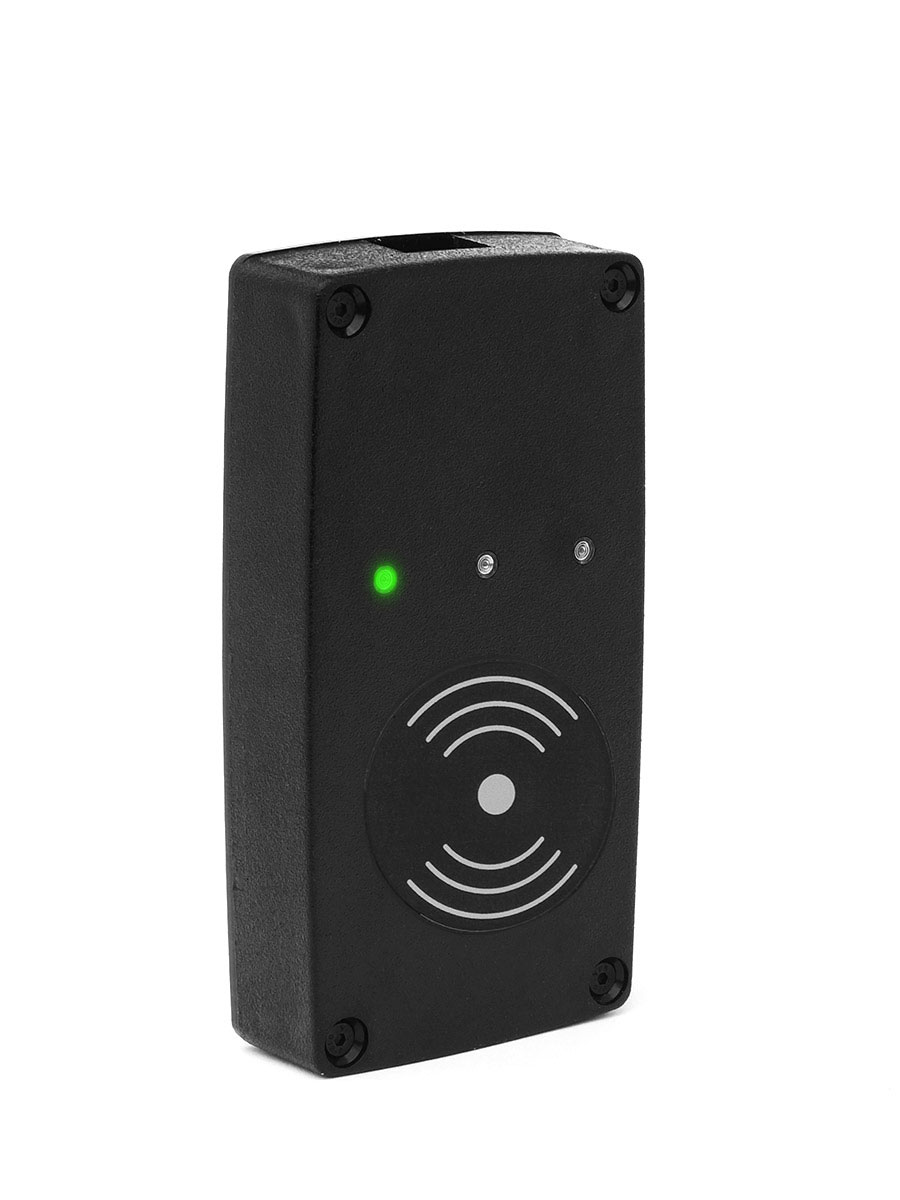
\includegraphics[scale=0.2]{orbit.jpg}
\centering
\caption{Gemini 2000 Orbit IP}
\centering
\end{figure}

\section{Python 3}
Python je interpretativni programski jezik nastao od strane Guido van Rossuma 1991. godine. Najčešće je zbog svoje jednostavnosti i proširivosti različitim bibliotekama popularan u različitim područjima razvoja. Neka od područja su:

\begin{itemize}
\item Skriptiranje - kao interpretativni jezik koristi se za podešavanje sustava te pisanje jednostavnih skripti za različite namjene
\item Matematika - zbog velikog izbora matematičkih bibilioteka Python je jezik koji se često koristi za statistiku i strojno učenje
\item Razvoj web aplkacija - poslužiteljski dio aplikacija sve više je razvijan u Pythonu. Interpretativni način rada iako nije najbrži dozvoljava brži razvoj i testiranje aplikacija. Također zbog mnogo razvojnih okvira koji nude brzi razvoj i proširivost
\end{itemize} 

Za razvoj ovog rada odabran je Python zbog svoje rasprostranjenosti, količine bibilioteka i neovisnosti o sustavu na kojem se izvršava. Python također karakterizira i čitljivost koda te kao takav je savršen za razvoj manjih projekata.

\begin{figure}[h]

\includegraphics[scale=0.5]{python.png}
\centering
\caption{Programski jezik Python}
\centering
\end{figure}

\section{TinyDB}
TinyDB je mala baza podataka orijentirana na dokumentima. Podaci se spremaju u jednu datoteku koja je zapisana u JSON formatu. Zbog malog broja informacija koje se moraju spremati u bazu, nema potrebe za bazama podataka koje imaju više mogućnosti, brže su, ali i zauzimaju više memorije kod izvršavanja.

\begin{figure}[h]

\includegraphics[scale=0.4]{tinydb.png}
\centering
\caption{Baza podataka TinyDB}
\centering
\end{figure}

\section{Vim}
Vim je tekstualni editor koji zbog svoje velike mogućnosti proširenja i efikasnosti kod pisanja programa je savršeni alat za razvijanje programskih rješenja. Neke od njegovih glavnih značajka su:
\begin{itemize}
\item dosljedno, više razinsko stablo poništavanja
\item veliki izbor nadogradnji
\item podrška za stotine programskih jezika i datotečnih formata
\item snažna pretraga i promjena teksta
\item mogućnost integracija s mnogo alata
\end{itemize}

\begin{figure}[h]

\includegraphics[scale=0.1]{vim.png}
\centering
\caption{Tekstualni editor Vim}
\centering
\end{figure}

\section{Git}
Git je besplatan distiribuirani sustav za upravljanje izvornim kodom nastao 2005. godine od strane Linus Torvalds. Git kao alat služi da bi se efikasno i lako pratile promjene nastale u razvoju programskog kod.\par
U ovom projektu git-ova glavna svrha je bila spremanje promjena te mogućnost lakog dohvaćanja istog na drugom računalu više nego kao sustav za kontrolu verzijama. Upravitelj repozitorija korišten je GitHub.

\begin{figure}[h]

\includegraphics[scale=0.2]{git.jpg}
\centering
\caption{Sustav za upravljanje izvornim kodom Git}
\centering
\end{figure}

\chapter{Beskontaktna tehnologija niže frekvencije (\textbf{NFC})}
Beskontaktna tehnologija niže frekvencije, (eng. \textit{Near field communication}) ili skraćeno NFC je vrsta beskontaktne komunikacije između uređaja poput mobilnih telefona i beskontaktnih kartica. Beskontaktna komunikacija dozvoljava komunikaciju na male udaljenosti bez potrebe da uređaji dolaze u neposredni doticaj. \par
NFC dozvoljava uređaju, koji služi kao čitač, tj. ispitivač, proizvodi aktivno radio frekvenciju što mu dozvoljava da komunicira s ostalim NFC kompatibilnim uređajima ili karticama. Pasivni uređaji poput beskontaktnih kartica i oznaka, imaju spremljenu informaciju te tu informaciju razmjenjuju s čitačima, ali ne dozvoljavaju čitanje informacija drugih uređaja. Kod komunikacije dva aktivna uređaja postoji obostrana komunikacija slanja i primanja informacija.\par 
Integracija beskontaktnih tehnologija u kreditne, putničke i kuponske kartice dozvoljava korisnicima da obavljaju plaćanja, ukrcavanje na javni prijevoz i razmjenu informacija preko jednostavnog  približavanja kartica. Također postoji mogućnost integracije više usluga preko mobilnih telefona te tako eliminirati korištenje različitih kartica za različite usluge.\par 
U današnje vrijeme sve više poduzeća implementira beskontaktne tehnologije u svoje usluge, uključujući implementacije virtualnih kartica koje dozvoljavaju plaćanjem na kartičnim terminalima pomoću mobilnih telefona.

\begin{figure}[h]
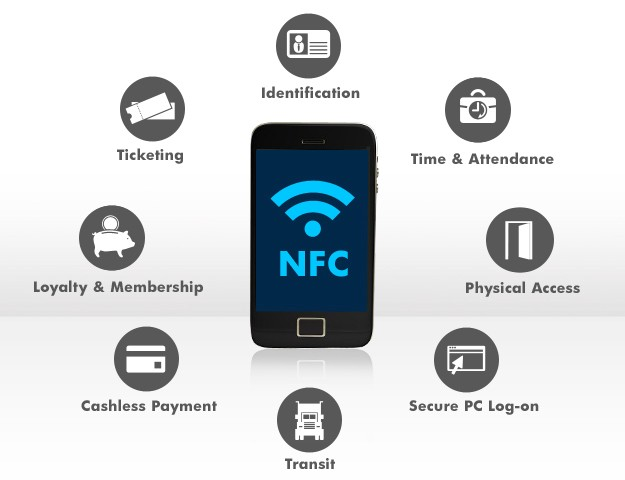
\includegraphics[scale=0.4]{nfcuse.jpeg}
\centering
\caption{Upotreba NFC-a}
\centering
\end{figure}

\section{Povijest}
Beskontaktna tehnologija niže frekvencije postoji na temeljima radio-frekvencijske identifikacije (RFID). NFC je podset RFID-a s kraćim dometom zbog sigurnosnih razloga.\par 
2004. godine Nokia, Sony i Philips zajedno su formirali NFC Forum. Njihov zajednički cilj je bio promoviranje sigurnosti, jednostavnosti korištenja i popularnosti beskontaktne tehnologije niže frekvencije. Zaduženje Foruma je održavanje standarda koji dozvoljava da tehnologija može funkcionirati između sva uređaja. Ako netko želi proizvesti NFC uređaj potrebno je slijediti standarde postavljene od strane NFC Foruma. To osigurava da korisnik s bilo kojim NFC uređajem može komunicirati s nekim drugim NFC uređajem.\par
Iako je NFC Forum formiran 2004. godine, prve specifikacije za NFC oznake su se pojavile 2006. godine. NFC oznake su mali objekti koji sadrže informacije koje NFC čitaći mogu pročitati. Informacije na oznakama se u većini slučajeva mogu samo čitati, ali postoje i oznake u koje se mogu upisati nove ili promijeniti stare informacije.\par 
Prvi mobilni telefon koji je sadržavao NFC sposobnosti je bila Nokia 6131 NFC predstavljena 2006. godine. Sazrijevanjem tehnologije dolazile su i nove specifikacije koje su osim podržavanja plaćanja dozvoljavale i razmjenu slika, videa i ostalih informacija. Danas je NFC tehnologija dostupna na većini mobilnih uređaja, od telefona, pametnih satova do integracije u automobile.

\begin{figure}[h]

\includegraphics[scale=1.0]{nfc.png}
\centering
\caption{NFC Forum}
\centering
\end{figure}

\section{Tehnološki standard}
Kada se razvijaju NFC uređaji potrebno je pratiti NFC standarde. Standardi postoje da sve vrste NFC uređaja mogu međusobno komunicirati kako oni dizajnirani u prošlosti tako i u budućnosti. Postoje dvije vrste glavnih specifikacija za NFC tehnologiju:
\begin{itemize}
\item ISO/IEC 14443 koja definira identifikacijske kartice koje spremaju informacije, poput NFC oznaka
\item ISO/IEC 18000-3 koja definira radio-frekvencijsku identifikacijsku komunikacijsko NFC uređaja
\end{itemize}\par 
ISO/IEC 18000-3 je internacionalni standard za sve uređaje koji komuniciraju bežično na frekvenciji 13.56MHz. Uređaji trebaju biti na minimalnoj udaljenosti od 4cm prije nego dolazi razmjene informacija. Ovi standardi opisuju način na koji čitač i NFC oznaka s koje se čita trebaju komunicirati međusobno.\par
Čitač šalje signal oznaci. Ako su uređaji dovoljno blizu jedan drugom oznaka postaje napajana preko signala čitača. To dozvoljava da oznaka bude malena i bez potrebe da sadrži bateriju ili svoj vlastiti izvor napajanja.\par
Ta dva uređaja kreiraju visoko frekvencijsko magnetsko polje između zavojnica uređaja. Jednom kada je polje uspostavljeno, dolazi do konekcije i razmjene informacija između čitača i oznake. Čitač šalje prvu poruku oznaci kako bi doznao vrstu komunikacije koju oznaka koristi, tip A ili tip B. Kada oznaka odgovori čitač šalje prvu naredbu koja mora odgovarati specifikaciji.\par 
Oznaka nakon primitka naredbe provjerava je li ona ispravna. Ako nije, oznaka ne odgovara. U protivnom odgovara s zahtijevanom informacijom. Kod  nekih komunikacija poput kartičnih plaćanja dolazi do uspostave sigurnog komunikacijskog kanala i sve informacije poslane su enkriptirane.\par 
NFC oznake rade na principu da u jednom trenutku mogu samo primati ili slati informacije, dok čitači mogu primati informacije i slati naredbe istovremeno. Naredbe se šalju s čitaća preko modulacijskog faznog podrhtavanja (eng. \textit{phase jitter modulation}) (PJM) kako bi modificirao okružujuće polje i poslao signal. Oznaka odgovara koristeći induktivnost kako bi poslala naboj preko svojih zavojnica.\par 
Prateći ove specifikacije osiguravamo da svi NFC uređaji mogu međusobno komunicirati.

\begin{figure}[h]
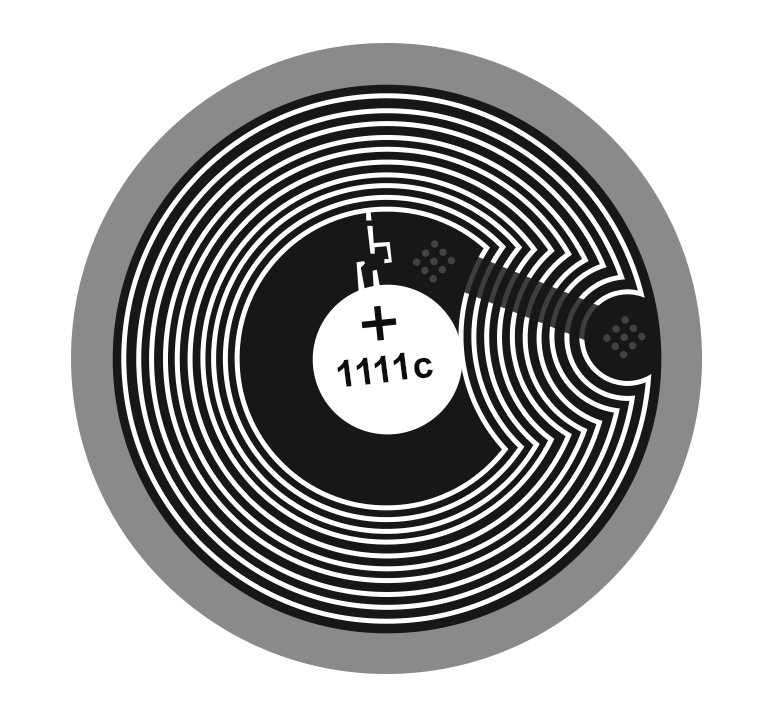
\includegraphics[scale=0.2]{nfctag.png}
\centering
\caption{Unutrašnjost NFC oznake}
\centering
\end{figure}

\section{Sigurnosni problemi}
Korisnici NFC tehnologije se naravno pitaju koji su sigurnosni rizici pogotovo oni koji ju koriste za kartična plaćanja. Jesu li njihove informacije sigurne i otporne na krađu? U nastavku su neki od sigurnosnih problema koji se mogu pojaviti i kako NFC tehnologija ih sprječava.
\subsection{Prisluškivanje}
Prisluškivanje se dešava kada osoba prati komunikaciju između čitača i oznaka. Nije potrebno pratiti svaki signal da bi se prikupila privatna informacija. Postoje dvije metode kako spriječiti prisluškivanje:
\begin{itemize}
\item udaljenost na kojoj NFC radi. Kako NFC radi na maloj udaljenosti prisluškivanje se može desiti na jako malom području.
\item Sigurni kanali. Kada je uspostavljen sigurni kanal, sve informacije koje se razmjenjuju su enkriptirane i samo ovlašteni uređaji ih mogu dekriptirati. Potrebno je samo provjeriti koriste li čitaći sigurne kanale.
\end{itemize}
\subsection{Korupcija i manipulacija podataka}
Korupcija i manipulacija se dešavaju kada osoba manipulira informacijama koje se šalju čitaću ili posreduje informacijama tako da budu iskvarene i beskorisne kada dođu do čitača. Kako bi se spriječila korupcija i manipulacija koriste se sigurni kanali. Neki uređaji mogu prepoznati takve napade i spriječiti ih prije nego što se dogode.
\subsection{Presretanje}
Presretanje je slično manipulaciji podataka. Kod presretanja postoji posrednik koji čita, mijenja sve informacije koje se razmjenjuju između čitača i oznake. Ovakva vrsta napada je složena za izvesti i rjeđe se dešava. Kako bi se spriječio jedan uređaj mora djelovati aktivno, a drugi pasivno. To znači da jedan šalje, a drugi prima informacije umjesto da oba šalju i primaju informacije.
\subsection{Krađa}
Ako dođe do krađe mobilnog telefona ili kartice kradljivac može lako oponašati osobu te tako dobiti pristup plaćanjima i ulazima. Zato je potrebno upotrijebiti dodatne mjere sigurnosti kao postavljanje sigurnosnih lozinka na svoje mobilne uređaje ili u slučaju kartica i oznaka prijaviti krađu svim administratorima sustava kod kojih je ta kartica ili oznaka zabilježena.

\section{Jedinstveni identifikacijski broj (UID)}


\chapter{Arhitektura i dizajn sustava}
U ovome poglavlju objašnjena je cijela struktura sustava za kontrolu ulaza korištenjem beskontaktnih kartica. Sustav se sastoji od:
\begin{itemize}
\item sustava za autentifikaciju
\item Orbit IP čitača
\end{itemize}

Sustav je zamišljen kao jednostavan sustav za kontrolu ulaza koji omogućuje autentifikaciju preko beskontaktnih kartica koje sadrže NFC tehnologiju. Naravno postoji mogućnost autentifikacije i mobilnim telefonima koji podržavaju NFC. \par 

\section{Struktura programske podrške}
Programska podrška se sastoji od skripte za pokretanje aplikacije za kontrolu ulaza, aplikacije za kontrolu ulaza, aplikacije za unošenje identifikatora u bazu podataka i baze podataka.
\begin{figure}[h]
\dirtree{%
 .1 NFC\_Handler.
 .2 database\_input.py.
 .2 db.json.
 .2 nfc\_handler.py.
 .2 startup.sh. 
}
\caption{Struktura programske podrške}
\end{figure}

\section{Baza podataka}
Baza podataka je jednostavna datotečna baza u JSON formatu. Nalazi se u datoteci \textbf{db.json}.	\par
JSON je tekstualni format koji je jezično neovisan, ali koristi konvencije koje su poznate većini programera.\par
JSON podaci se spremaju u obliku \{'ime' : 'vrijedost'\} koje predstavljaju jedan objekt. Objekti su međusobno odijeljeni zarezima.\par 
Kod baze podataka ovog rada postoji glavni objekt \textbf{\_default} koji predstavlja korijen te sadrži objekte nizane   sljednim brojevima. Svaki broj sadrži objekt imena \textbf{uid} (eng. \textit{Unique ID}) i vrijednost koja predstavlja identifikacijski broj NFC oznake. Identifikacijski broj oznake sadrži vrijednosti zapisane u \textbf{heksadecimalnom} formatu, a veličina identifikatora ovisi o proizvođaču, ali je najčešće veličine 7 bajta.

\begin{lstlisting}[language=json,firstnumber=1]
{"_default": {
  "1": {"uid": "AEF056"}, 
  "2": {"uid": "123456"},
  "3": {"uid": "555555"},
  "4": {"uid": "31053B71"},
  "5": {"uid": "123456"}
}}

\end{lstlisting}
\captionof{lstlisting}{Primjer izgleda datoteke db.json}

\section{Autentifikacija}
Autentifikacija korisnika se provodi preko aplikacije \textbf{nfc\_handler.py}.\par
Tijek izvršavanja programa je sljedeći:
\begin{itemize}
\item Kreiranje HTTP servera
\item Učitavanje baze podataka
\item Čekanje na zahtjev čitača
\item Korisnik prilaže NFC karticu
\item Čitač pošalje zahtjev
\item Aplikacija parsira dobiven zahtjev
\item Aplikacija provjerava u bazi podataka 
   \begin{itemize}
   \item Postoji UID, vrati čitaču da otvori vrata
   \item Ne postoji UID, vrati čitaču da ne otvara vrata
   \item Nema UID u poslanom zahtjevu, pošalji prazan odgovor
   \end{itemize}
\item Vrati se na čekanje zahtjeva
\end{itemize}

\begin{figure}[h]
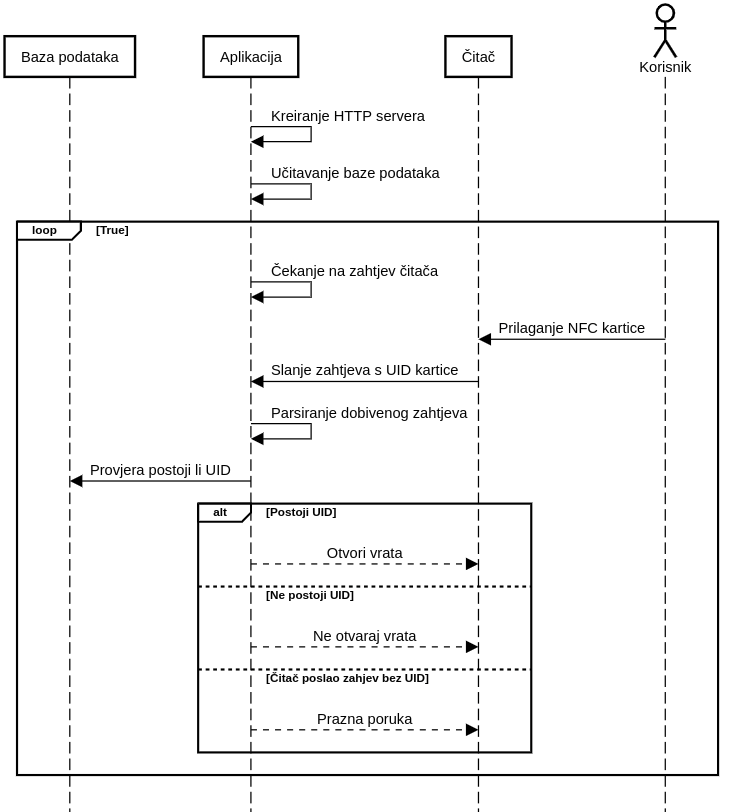
\includegraphics[scale=0.5]{sequence.png}
\centering
\caption{Sekvencijski dijagram sustava}
\centering
\end{figure}

\subsection{Inicijalizacija aplikacije}
Aplikacija se incijalizira uključivanjem iz biblioteka:
\begin{itemize}
\item \textbf{http.server} klase:
	\begin{itemize}
	\item HTTPServer
	\item BaseHTTPRequestHandler
	\end{itemize}
\item \textbf{tinydb} klase
	\begin{itemize}
	\item TinyDB
	\item Query
	\end{itemize}
\item \textbf{datetime}, klasu datetime
\item \textbf{socket}
\end{itemize}

Postavlja \textbf{HOST\_NAME} i \textbf{PORT\_NUMBER}. Te varijable su postavljene na IP adresu '192.168.7.191' i vrata 80  jer čitač zadano šalje svoje zahtjeve na tu adresu i vrata.\par
Dolazi do inicijalizacije web poslužitelja i dohvaćanje baze podataka. Nakon toga aplikacija čeka na zahtjeve od čitača.

\begin{figure}[h]
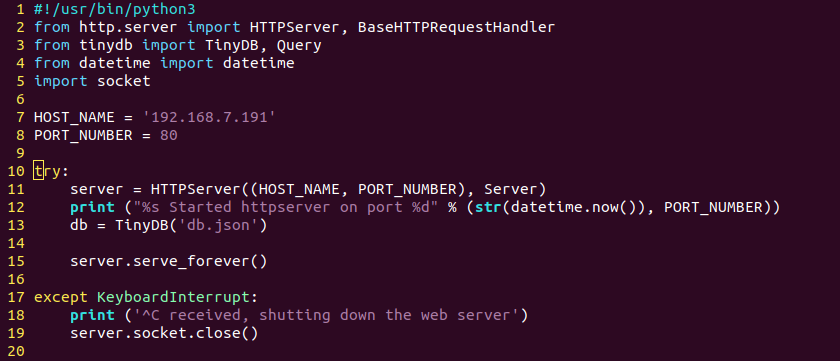
\includegraphics[scale=0.5]{init.png}
\centering
\caption{Inicijalizacija aplikacije}
\centering
\end{figure}

\subsection{Parsiranje zahtjeva}
Kada aplikacija dobije zahtjev od čitača, čitač sve informacije šalje putem URL-a. Zato je potrebno parsirati URL i pronači UID. Za to služi funkcija \textbf{handle\_nfc}.\par
UID se pronalazi prvo traženjem njegove duljine u bajtima, a zatim se traži identifikacijski broj.\par 
Funkcija vraća ili duljinu UID-a i UID ili vrijednosti False, False ovisno o uspješnosti pronalaska istih u zahtjevu.

\begin{figure}[h]
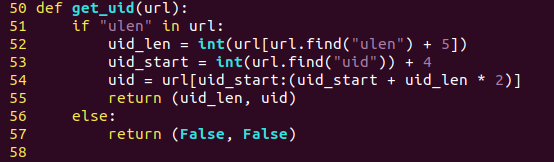
\includegraphics[scale=0.5]{parsiranje.png}
\centering
\caption{Parsiranje zahtjeva}
\centering
\end{figure}

\subsection{Provjera baze podataka}
Nakon parsiranja zahtjeva dolazimo do provjere postoji li dobiveni UID u bazi podataka. Koristimo funkciju \textbf{handle\_nfc}.\par 
Provjera se izvršava preko instancirane baze \textbf{db} i njene funkcije \textbf{search}. \par 
Ako postoji UID u bazi zabilježavamo vrijeme, otvaranje vrata i UID te vraćamo \textbf{'Open'}.\par 
Ako ne postoji UID u bazi zabilježavamo vrijeme, neautoriziran pristup i UID te vraćamo \textbf{'Close'}.\par 
Ako u zahtjevu nije postojao UID, tj. čitač je poslao svoj dijagnostički zahtjev, vraćamo \textbf{'PING'}. 
\begin{figure}[h]
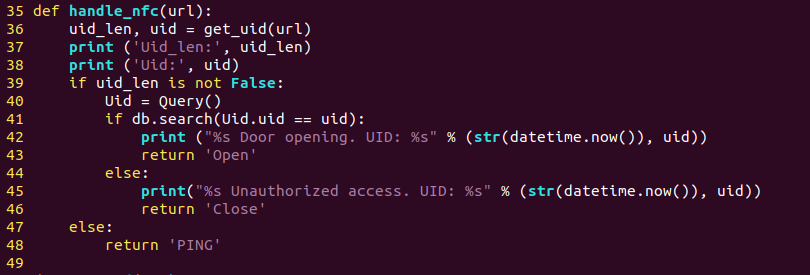
\includegraphics[scale=0.5]{baza.png}
\centering
\caption{Provjera baze podataka}
\centering
\end{figure}

\subsection{Obrada zahtjeva}
Klasa Server čeka HTTP zahtjev od strane čitača. Kada čitač pošalje zahtjev klasa šalje URL zahtjeva prethodno opisanoj funkciji \textbf{handle\_nfc}. \par
Kada funkcija vrati povratnu informaciju ovisno o njoj šalje čitaču odgovor.\par 
Nakon slanja odgovora aplikacija se vraća u stanje čekanja zahtjeva.



\begin{figure}[h]
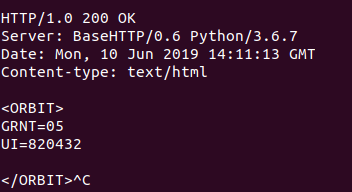
\includegraphics[scale=0.6]{grant.png}
\centering
\caption{Odgovor kod uspješne autentifikacije}
\centering
\end{figure}

\begin{figure}[h]
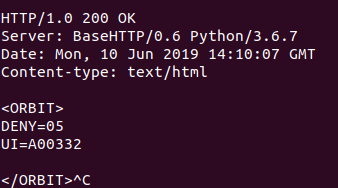
\includegraphics[scale=0.6]{deny.png}
\centering
\caption{Odgovor kod neuspješne autentifikacije}
\centering
\end{figure}

\begin{figure}[h]
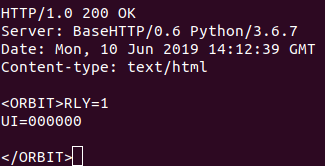
\includegraphics[scale=0.6]{ping.png}
\centering
\caption{Odgovor kod dijagnostičkog zahtjeva}
\centering
\end{figure}

\begin{figure}[H]
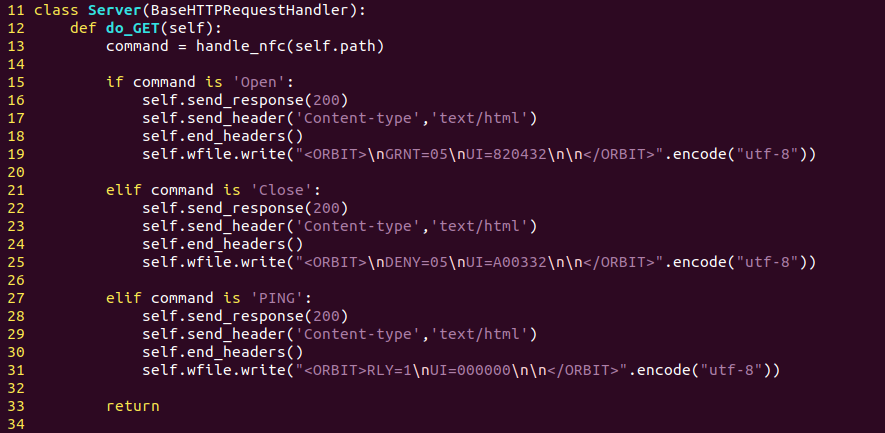
\includegraphics[scale=0.5]{server.png}
\centering
\caption{Obrada zahtjeva}
\centering
\end{figure}

\newpage

\section{Implementacija}
Čitač i uređaj na kojoj se pokreće poslužiteljska aplikacija, Raspberry Pi Model 2 B, komuniciraju putem Ethernet priključka.\par 
Čitač je također i napajan preko Ethernet priključka te je za njegov rad potreban PoE mrežni preklopnik ili PoE ubrizgivač. Kod implementacije rada koristio se Mikrotik Gigabit PoE ubrizgivač u koji se dovodi upredena parica i 48V istosmjerni pretvornik. 

\begin{figure}[h]
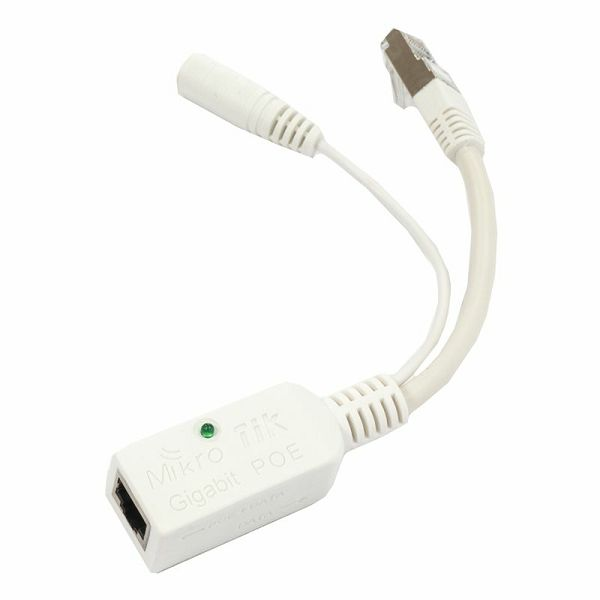
\includegraphics[scale=0.3]{poe.jpg}
\centering
\caption{Mirkotik Gigabit PoE ubrizgivač}
\centering
\end{figure}

Čitač i Raspberry Pi povezani su međusobno bez upotrebe usmjeritelja. Zato je potrebno na Raspberry Pi-u uspostaviti mrežu. Mreža se uspostavlja preko skripte \textbf{startup.sh}.\par 
Skripta također šluži za instalaciju baze podataka \textbf{TinyDB} i pokreće poslužiteljsku aplikaciju \textbf{nfc\_handler.py}.

\begin{figure}[h]
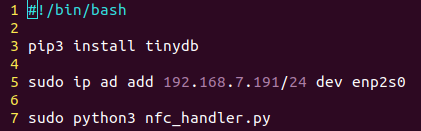
\includegraphics[scale=0.6]{skripta.png}
\centering
\caption{Bash skripta startup.sh}
\centering
\end{figure}

Zadnja dio sustava je elektronička brava koja otvara bravu kada dobije napon od 12V. Napon dobiva iz čitača koji putem releja kod odgovora od poslužiteljske aplikacije daje napon kroz žice. 

\begin{figure}[h]
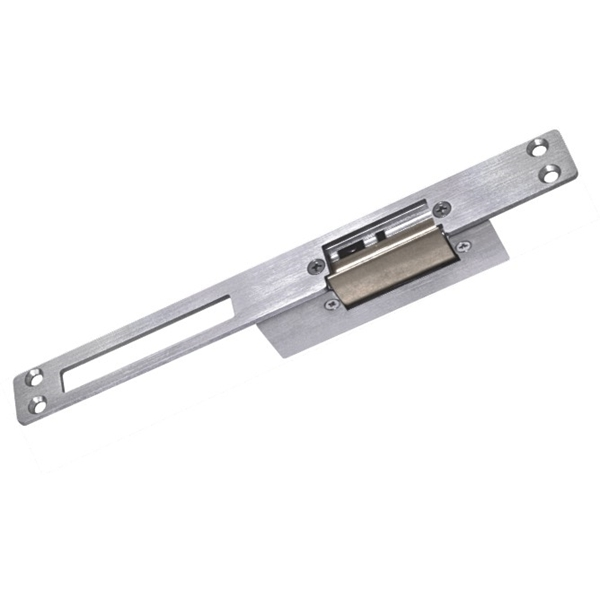
\includegraphics[scale=1]{brava.jpg}
\centering
\caption{Elektronička brava}
\centering
\end{figure}

\begin{figure}[h]
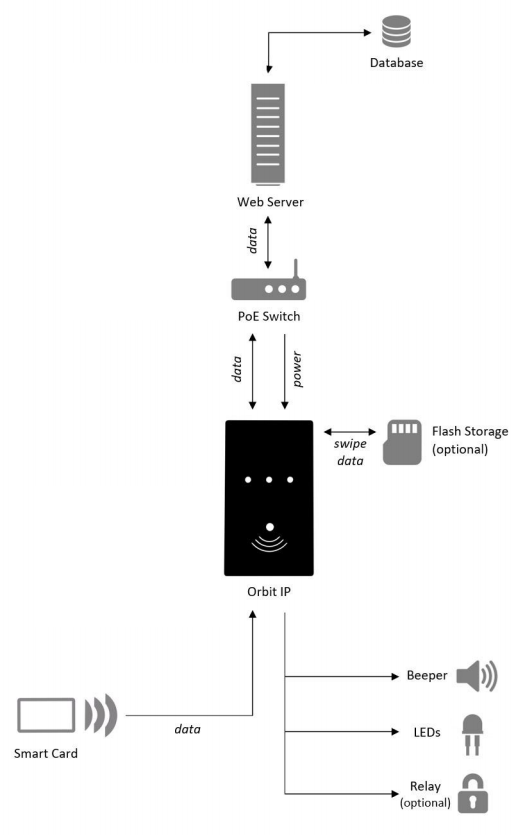
\includegraphics[scale=0.5]{arhitektura.png}
\centering
\caption{Shema sustava}
\centering
\end{figure}


\chapter{Zaključak}
Zaključak.

\bibliography{literatura}
\bibliographystyle{fer}

\begin{sazetak}
Sažetak na hrvatskom jeziku.

\kljucnerijeci{Ključne riječi, odvojene zarezima.}
\end{sazetak}

% TODO: Navedite naslov na engleskom jeziku.
\engtitle{Title}
\begin{abstract}
Abstract.

\keywords{Keywords.}
\end{abstract}

\end{document}
